\title{Math 239 Fall 2023 Tutorial Questions Week 8}

\date{2023 Nov. 9/10}
\maketitle

\begin{enumerate}

    \question{Exotic Cubes} Let $C_{n,m}$ be the graph where the vertices are the elements of $\{ 0, 1 , \cdots, m-1\}^n$, and where there is an edge between $v_1$ and $v_2$ iff $v_1 $ and $v_2$ differ by exactly $1$ in exactly one coordinate. For example if $n=2$ and $m=3$ the vertex $(1,2)$ to the vertices $(0,2) , (2,2) , (1,1)$.
    \begin{enumerate}
        \item Draw $C_{2,3}$.
        \item Is $C_{n,m}$ bipartite?
        \item What is the maximum degree of a vertex in $C_{n,m}$? What about the minimum?
        \item (hard, attempt other questions first) What is the number of edges in $C_{n,m}$?
    \end{enumerate}
    
    % We write $K_{n_1 , \cdots, n_k}$ to be the graph with $|V_j| = n_j$, and $uv \in E$ iff $u \in V_a, v \in V_b$ where $a \neq b$ (ie if two vertices are in different parts there is an edge between them). Note that $K_{n_1 , \cdots, n_k}$ has $n_1 + \cdots + n_k$ vertices. This is called the \textbf{complete $k$-partite graph on $n_1 , \cdots, n_k$ vertices}.

    
    
    
    \question{Find the Mistake} The following is a false statement and a false proof. Identify the error in the provided proof and consider how to avoid making this mistake in general. Can you think of a way to make the theorem true? If so, prove it. 
    \\
    \textbf{Non-theorem:} If $G$ is a graph with $|V(G)|\geq 4$ and minimum degree at least $2$, then $G$ contains a cycle of length at least $4$.
    \\
    \textbf{Non-proof:} We proceed by induction on $|V(G)|$. We begin with the base case: Let $G$ be a graph with four vertices and minimum degree at least $2$. Suppose for a contradiction that $G$ does not contain a cycle of length $4$. Since $G$ has minimum degree at least two, it follows that $G$ contains a cycle: and since $G$ does not contain a cycle of length $4$, it therefore contains a cycle of length $3$. Let $v$ be the vertex not in this cycle of length three. Since $G$ has minimum degree at least $2$ and $|V(G)|=4$, it follows that $v$ is adjacent to at least two vertices in this cycle. Then $G$ does contain a cycle of length $4$, a contradiction. Thus the base case holds. To prove the inductive step, let $H$ be a graph on $n-1$ vertices for which the theorem holds. Construct a new graph $G$ on $n$ vertices by adding a new vertex to $H$ with at least two incident edges. Since $H$ contains a cycle of length $4$ by induction, $G$ contains a cycle of length $4$ and the result holds. 
    
    
    \question{Pr{\"u}fer Codes} Let $n \ge 3$, and suppose we have a tree on vertex set $\{1, \dots, n\}$. We can construct a sequence of elements from $\{1, \dots, n\}$ algorithmically as follows:
    \begin{enumerate}[label=\arabic*)]
        \item Check to make sure the tree has more than a single edge. If not, terminate.
        \item Find the leaf with the smallest label. Add the label of its neighbor to the sequence. Delete the leaf from the graph and repeat.
    \end{enumerate}
    Notice that this will produce a sequence of length $n - 2$, as we're terminating the algorithm when we have a single edge (two vertices) left. The sequence we get from this algorithm is called a Pr{\"u}fer sequence.

    \begin{enumerate}
        \item Write the Pr{\"u}fer sequences for the following trees:

        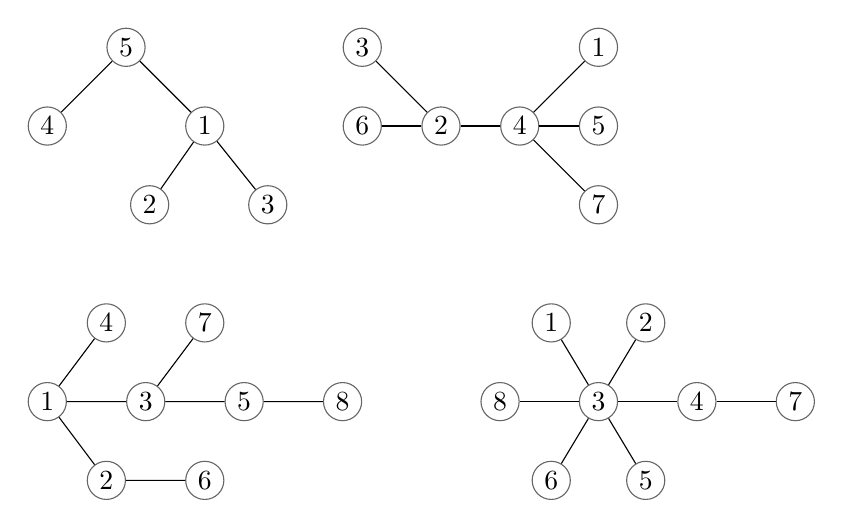
\begin{tikzpicture}[shorten >=1pt,->]
  \tikzstyle{vertex}=[circle,draw=black!60,minimum size=12pt,inner sep=2pt]
  \node[vertex] (G_4) at (-1,-1) {4};
  \node[vertex] (G_5) at (0,0)   {5};
  \node[vertex] (G_1) at (1,-1)  {1};
  \node[vertex] (G_2) at (0.3,-2)  {2};
  \node[vertex] (G_3) at (1.8,-2)  {3};
  \draw (G_4) -- (G_5) -- (G_1) -- (G_2) -- cycle;
  \draw (G_1) -- (G_3) -- cycle;

\node[vertex] (G_6') at (3,-1) {6};
\node[vertex] (G_3') at (3,0) {3};
  \node[vertex] (G_2') at (4,-1)   {2};
  \node[vertex] (G_4') at (5,-1)  {4};
  \node[vertex] (G_1') at (6,0)  {1};
  \node[vertex] (G_5') at (6,-1)  {5};
  \node[vertex] (G_7') at (6,-2)  {7};
  \draw (G_6') -- (G_2') -- (G_4') -- (G_5') -- cycle;
  \draw (G_4') -- (G_1') -- cycle;
  \draw (G_3') -- (G_2') -- cycle;
  \draw (G_4') -- (G_7') -- cycle;

  \node[vertex] (G_4'') at (-0.25,-3.5) {4};
  \node[vertex] (G_1'') at (-1,-4.5)   {1};
  \node[vertex] (G_2'') at (-0.25,-5.5)  {2};
  \node[vertex] (G_6'') at (1,-5.5)  {6};
  \node[vertex] (G_3'') at (0.25,-4.5)  {3};
  \node[vertex] (G_7'') at (1,-3.5)  {7};
  \node[vertex] (G_5'') at (1.5,-4.5)  {5};
  \node[vertex] (G_8'') at (2.75,-4.5)  {8};
  \draw (G_1'') -- (G_4'') -- cycle;
  \draw (G_6'') -- (G_2'') -- (G_1'') -- (G_3'') -- (G_5'') -- (G_8'') -- cycle;
  \draw (G_3'') -- (G_7'') -- cycle;

  \node[vertex] (H_3) at (6,-4.5) {3};
  \node[vertex] (H_1) at (5.4,-3.5)   {1};
  \node[vertex] (H_2) at (6.6,-3.5)   {2};
  \node[vertex] (H_4) at (7.25,-4.5)  {4};
  \node[vertex] (H_7) at (8.5,-4.5)  {7};
  \node[vertex] (H_8) at (4.75,-4.5)  {8};
  \node[vertex] (H_6) at (5.4,-5.5)   {6};
  \node[vertex] (H_5) at (6.6,-5.5)   {5};
  
  \draw (H_8) -- (H_3)  -- (H_4)  -- (H_7) -- cycle;
  \draw (H_1) -- (H_3)  -- (H_5)  -- cycle;
  \draw (H_2) -- (H_3)  -- (H_6)  -- cycle;
    
\end{tikzpicture}

\hfill
                
        \item Can any sequence of $n-2$ numbers from $\{1, \dots, n\}$ be the Pr{\"u}fer sequence of a tree on $n$ vertices? Construct an algorithm for building a labeled tree out of a given sequence, or explain why it's not possible. 

        \item Use Pr{\"u}fer sequences to count the number of labelled trees on $n$ vertices. (Hint: The algorithm you wrote in part (b) gives you a mapping that is the inverse of the mapping from labeled trees to their Pr{\"u}fer sequences. You do not need to prove that it's a bijection.)

        \item (hard, attempt other questions first) Prove that the algorithm gives us a bijective mapping. 
    \end{enumerate}
    
    
    \question{Spanning Tree} Let $e$ be an edge in a connected graph $G$. Prove that $e$ is a bridge in $G$ if and only if $e$ is in every spanning tree of $G$.

    \question{Bonus: Complete $k$-partite Graphs} We say a graph $G=(V,E)$ is \textbf{$k$-partite} if we can partition $V = V_1 \sqcup \cdots \sqcup V_k$ ($\sqcup$ indicates \textit{disjoint} union, and the $V_j$ are called \textit{parts}) such that there are no edges between distinct elements of $V_j$ (where $j = 1, \cdots, k$). Find a tight bound on the number of edges in a $k$-partite graph with $kn$ vertices, and say when this tight bound occurs.
\end{enumerate}